\documentclass[11pt,oneside]{book}
\usepackage[margin=1in]{geometry}
\usepackage{amsmath,amssymb,amsthm}
\usepackage{xcolor}
\usepackage{enumitem}
\usepackage{tikz}
\usetikzlibrary{arrows.meta,positioning,calc}
\usepackage{graphicx}
\usepackage[hidelinks]{hyperref}
\usepackage{listings}

\newtheorem{definition}{Definition}
\newtheorem{example}{Example}
\newtheorem{proposition}{Proposition}
\newtheorem{theorem}{Theorem}

\tikzset{compartment/.style={draw, minimum width=1cm, minimum height=1cm}}

\lstset{
  language=Python,
  basicstyle=\ttfamily\small,
  columns=fullflexible,
  breaklines=true,
  showstringspaces=false,
  commentstyle=\itshape,
}

\title{Mathematical Models of Infectious Diseases}
\author{Yair Daon}
\date{\today}

\begin{document}
\maketitle
\tableofcontents

\documentclass[11pt]{article}
\usepackage[margin=1in]{geometry}
\usepackage{amsmath,amssymb}
\usepackage{enumitem}

\title{Module 0: Introduction}
\author{}
\date{}

\begin{document}
\maketitle

\noindent\textbf{Note on this transcription.} This is a best-effort translation of a paragraph of fast Hebrew cursive. It was hard to read; uncertain words/phrases are marked \emph{[uncertain]} below --- please correct these, since it is your own handwriting.

\section{Course planning notes (partial, best-effort translation)}

\begin{itemize}
  \item Header: ``Motivation: [\emph{uncertain}] of 5 leading global causes of [\emph{uncertain, likely} death / morbidity and mortality]'' (text runs off the edge of the page).
  \item A note involving the word \emph{morbidity} and the top global causes of death/disease burden.
  \item A phrase about types of infection / contagion (\emph{ease of transmission?}) --- \emph{[uncertain]}.
  \item A crossed-out idea mentioning ``30\%'' and ``coping/dealing with [something]'' --- struck through, apparently discarded.
  \item A second crossed-out line --- \emph{[illegible]}.
  \item ``Book: Keeling and Rohani.'' (reference to the course textbook)
  \item A note about ``explaining a paradox'' --- \emph{[uncertain]}.
  \item ``Preparation: a day, and an exercise/summary of an idea.'' --- \emph{[uncertain]}.
  \item ``Presentation: SIR model, [\emph{uncertain, possibly} Corona].''
\end{itemize}

\end{document}

\chapter{Calculus}

\section{Exponents and logarithms}
The exponential function is
\[
e^x = 1 + x + \frac{x^2}{2} + \frac{x^3}{3!} + \cdots
\]
The function $\log$ is the inverse of the exponential:
\[
\log e^x = x
\]


For small $x$, truncating after the linear term gives the useful approximation
\[
e^x \approx 1+x \qquad (x \text{ small}).
\]
Since $\log$ is the inverse of $e^x$, the same approximation, read the other way, gives
\[
\log(1+x) \approx x \qquad (x \text{ small}).
\]

\subsection{Identities}
\begin{align*}
  \left (e^x\right )^y &= e^{xy} \\
  \log x^y &= y \log x \\
  e^{x+y} &= e^x e^y.
\end{align*}
%% Derivative of the exponential:
%% \[
%% \frac{d}{dx}e^x = e^x, \qquad \frac{d}{dx}e^{kx} = k\,e^{kx}.
%% \]

\section{The derivative as a linear approximation}
\[
y+\Delta y = y(x+\Delta x) \approx y(x) + y'(x)\Delta x
\quad\Longrightarrow\quad
\Delta y = y'(x)\Delta x.
\]
$y'(x)$ is called \emph{the derivative}; it is also written $\dfrac{dy}{dx}$.

\subsection{Multiplication by a scalar}
What is the derivative of $z(x) = y(\alpha x)$? By the linear approximation:
\[
z + \Delta z \approx z(x) + z'(x) \Delta x
\]
But, on the other hand, by the definition of $z$:
\begin{align*}
  z + \Delta z &= z(x+\Delta x)\\
  &= y(\alpha x + \alpha \Delta x) \\
  &=y(\alpha x) + y'(\alpha x) \alpha \Delta x \\
  &=z(x) + y'(\alpha x) \cdot  \alpha \Delta x
\end{align*}
Therefore
\[
z'(x) = \alpha y'(\alpha x)  
\]
We will see later what this means for change of units. In the
meantime, note a specific example: $(e^{\alpha x})' = \alpha e^{\alpha x}$.
\subsection{Other identities}
\begin{align*}
  &\text{Sum rule:}&& (y+z)'(x) = y'(x) + z'(x) \\
  &\text{Product / Leibniz rule:}&&   (yz)'(x) = y'(x)z(x) + y(x)z'(x) \\
  &\text{Chain rule:}&&   \left (y(z(x))\right )' = y'(z(x)) \cdot z'(x)
\end{align*}



%% Our main unit of measurement is time, denoted $t$, measured in (say)
%% days. Let $I_d(t)$ be the number of infected individuals in a population
%% after $t$ days have passed. Then $\dot{I}_d$ is the change in the number
%% of infections per day, i.e.~the rate of new infections. How many new
%% infections can we expect in a week? Clearly that number is $7
%% \dot{I}_d$! But why? What has happened here?

%% Denote $\tau = t / 7$ --- the number of \emph{weeks} passed. So
%% the number of infected individuals after $\tau$ weeks is
%% $I_w(\tau) = I_d(7\tau)$. Then the rate of new infections per
%% \emph{week} is:
%% \begin{align*}
%%   \frac{d I_{w}}{d\tau} &=  7 \frac{d I_d}{d t} 
%%  \end{align*}

%% So we conclude: converting time to units $7$ times coarser multiplies
%% the rate by $7$. In general, measuring $t$ in units $k$ times coarser
%% (so $\tau = t/k$) multiplies any rate by $k$:
%% \[
%% \frac{dI_\star}{d\tau} = k\,\frac{dI}{dt}.
%% \]


\section{The Fundamental Theorem of Calculus}
\[
\int_a^b y'(x)\,dx = y(b) - y(a).
\]

\subsection{Why this works}
Partition $[a,b]$ into $n$ steps $a=x_0<x_1<\cdots<x_n=b$, each of
width $\Delta x$. By the linear approximation of Section~2, each step
changes $y$ by $\Delta y_i = y(x_{i+1})-y(x_i)\approx y'(x_i)\Delta x$. Summing the
steps telescopes:
\begin{align*}
  \sum_{i=0}^{n-1} y'(x_i)\,\Delta x & \approx \sum_{i=0}^{n-1} \Delta y_i \\
  &= \sum_{i=0}^{n-1}\underbrace{\big(y(x_{i+1})-y(x_i)\big)}_{\Delta y_i} \\
  &= \big(y(x_1)-y(x_0)\big) + \big(y(x_2)-y(x_1)\big) + \cdots +
  \big(y(x_n)-y(x_{n-1})\big)\\
  &= y(x_n)-y(x_0) \\
  &= y(b)-y(a).
\end{align*}

\begin{example}
Since $\frac{d}{ds}\left(-\frac{1}{\lambda}e^{-\lambda s}\right) = e^{-\lambda s}$, for $\lambda>0$ (so that $e^{-\lambda s}\to 0$ as $s\to\infty$),
\[
\int_t^\infty e^{-\lambda s}\,ds
= \left[-\frac{1}{\lambda}e^{-\lambda s}\right]_t^\infty
= \left(-\frac{1}{\lambda}e^{-\lambda \cdot \infty} + \frac{1}{\lambda}e^{-\lambda t}\right)
= \frac{1}{\lambda}e^{-\lambda t}.
\]
\end{example}

\chapter{Probability}

\section{Sample spaces and events}

\begin{definition}
An \emph{experiment} is a process with uncertain outcome. The
\emph{sample space} $\Omega$ is the set of all possible outcomes. An
\emph{event} is a subset $A\subseteq\Omega$.
\end{definition}

\begin{example}
A susceptible individual has one contact with an infectious person.
\[
\Omega=\{\text{infected},\ \text{not infected}\}.
\]
$A=\{\text{infected}\}$ is an event.
\end{example}

\section{Set operations on events}

\begin{itemize}
  \item \textbf{Union} $A\cup B$: ``$A$ or $B$ occurs.''
  \item \textbf{Intersection} $A\cap B$: ``$A$ and $B$ occur.''
  \item \textbf{Complement} $A^c$: ``$A$ does not occur.''
  \item \textbf{Disjoint}: $A\cap B=\emptyset$ ($A$ and $B$ cannot occur together).
\end{itemize}

\begin{example}
$A=\{$infected with strain 1$\}$, $B=\{$infected with strain 2$\}$.
\begin{itemize}[nosep]
  \item $A\cup B$: infected with at least one strain.
  \item $A\cap B$: co-infected with both strains.
  \item $A^c$: not infected with strain 1.
\end{itemize}
\end{example}

\section{The probability function}

\begin{definition}[Axioms of probability]
$\Pr$ assigns to each event $A\subseteq\Omega$ a number $\Pr(A)\in[0,1]$ such that
\begin{itemize}[nosep]
  \item $\Pr(\Omega)=1$;
  \item for disjoint events $A,B$, $\ \Pr(A\cup B)=\Pr(A)+\Pr(B)$.
\end{itemize}
\end{definition}

Interpretation: $\Pr(A)$ is the long-run fraction of times $A$ occurs (e.g. $\Pr(\text{infection})=0.3$ means 30\% of exposed contacts result in infection).

\section{Probability of the complement}
A very useful identity is $\Pr(A^c) = 1-\Pr(A)$.

%% \begin{proposition}[Addition law]
%% $\Pr(A\cup B) = \Pr(A)+\Pr(B)-\Pr(A\cap B)$.
%% \end{proposition}

\section{Conditional probabilities}
\[
\Pr(A|B) := \frac{\Pr(A \cap B)}{\Pr(B)} \qquad \text{whenever $\Pr(B) > 0$.}
\]
\section{Independence}

\begin{definition}
Events $A$ and $B$ are \emph{independent} if
\[
\Pr(A \cap B) = \Pr(A)\,\Pr(B).
\]
\end{definition}

If moreover $\Pr(B)>0$, this is equivalent (by the definition of
conditional probability above) to $\Pr(A|B) = \Pr(A)$.

Interpretation: knowing that some of the events occurred gives no
information about whether the others occurred.

\begin{example}
A susceptible individual has $n$ contacts. Each contact independently
transmits infection with probability $c$. Let $A_i=\{\text{contact $i$
  transmits infection}\}$, so $\Pr(A_i)=q$. Avoiding infection on
all $n$ contacts is the event $A_1^c\cap\cdots\cap A_n^c$, so by
independence
\[
\Pr(\text{avoid infection}) = \prod_{i=1}^n \Pr(A_i^c) = (1-q)^n.
\]
\end{example}

\section{Random variables}

\begin{definition}
A \emph{random variable} $X$ is a function $X:\Omega\to\mathbb{R}$ assigning a number to each outcome.
\end{definition}

\begin{example}
$T=$ time until recovery.
\end{example}

\begin{definition}
The \emph{density} (pdf) of $X$ is a function $f\ge 0$ with $\displaystyle\int_{-\infty}^\infty f(x)\,dx=1$ such that
\[
\Pr(a\le X\le b)=\int_a^b f(x)\,dx.
\]
The \emph{expectation} is $E[X]=\int x f(x)\,dx$.
\end{definition}

\section{The exponential random variable}

Used to model waiting times: time to recovery, time until next contact, incubation period.

\begin{definition}
$T$ has an \emph{exponential distribution with rate $\lambda>0$}, written $T\sim\text{Exp}(\lambda)$, if
\[
f(t)=\lambda e^{-\lambda t}, \qquad t\ge 0.
\]
\end{definition}

The \emph{survival function} is the probability of not yet having recovered by time $t$:
\[
S(t) = \Pr(T>t) = \int_t^\infty \lambda e^{-\lambda s}\,ds = e^{-\lambda t}.
\]
Mean: $E[T]=1/\lambda$.

Interpretation: if $T$ is the infectious period and $T\sim\text{Exp}(\gamma)$, then $\gamma$ is the recovery \emph{rate} and $1/\gamma$ is the mean infectious period.

\section{The memoryless property}
\begin{proposition}
  If $T\sim\text{Exp}(\lambda)$, then $T$ is memoryless, i.e.~
  \[
  \Pr(T> t+s \mid T> t) = \Pr(T> s) \qquad \text{for all } s,t\ge 0.
  \]
\end{proposition}
Interpretation: given that an individual is still infectious at time
$t$, the probability they remain infectious for $s$ more days does not
depend on $t$. Time already spent infected gives no information about
time remaining --- the recovery rate is constant, with no ``aging'' or
``wearing out.''

\begin{proof}
\begin{align*}
  \Pr(T> t+s\mid T> t) &= \frac{\Pr(T> t+s \cap T > t)}{\Pr(T > t)}\\
  &= \frac{\Pr(T> t+s)}{\Pr(T> t)}\\
  &= \frac{e^{-\lambda(t+s)}}{e^{-\lambda t}}\\
  &= e^{-\lambda s} \\
  &= \Pr(T> s).
\end{align*}
\end{proof}

\section{Minimum of independent exponentials}

\begin{proposition}
  If $X\sim\text{Exp}(\lambda)$ and $Y\sim\text{Exp}(\eta)$ are
  independent, define $Z=\min\{X,Y\}$.
\[
Z\sim\text{Exp}(\lambda+\eta).
\]
\end{proposition}

Interpretation: if an infected individual leaves the infected class
either by recovering (rate $\gamma$) or by dying of unrelated causes
(rate $\mu$), independently, then the time spent in the infected class
is $\min(T_{\text{recovery}}, T_{\text{death}})\sim\text{Exp}(\gamma+\mu)$
--- whichever happens first --- with mean $1/(\gamma+\mu)$.

\begin{proof}
By independence
\begin{align*}
  \Pr(Z>t) &= \Pr(X>t)\,\Pr(Y>t) \\
  &= e^{-\lambda t}e^{-\eta t}\\
  &= e^{-(\lambda+\eta)t} \\
\end{align*}
which is indeed the survival function of $\text{Exp}(\lambda+\eta)$.
\end{proof}

\chapter{The Basic SIR Model}

\section{Compartments}

We assume infection is \emph{acute}: an individual is infected, then
is removed (recovers or dies) and stays removed. Three compartments:
\begin{itemize}[nosep]
  \item $S$ --- Susceptible: can become infected.
  \item $I$ --- Infected: currently infectious.
  \item $R$ --- Removed: no longer infectious, not reinfected.
\end{itemize}

%% \begin{center}
%% \begin{tikzpicture}[node distance=2.5cm, >=Stealth]
%%   \node[compartment] (S) {$S$};
%%   \node[compartment] (I) [right=of S] {$I$};
%%   \node[compartment] (R) [right=of I] {$R$};
%%   \draw[->] (S) -- (I);
%%   \draw[->] (I) -- (R);
%% \end{tikzpicture}
%% \end{center}

We write $X,Y,Z$ for the \emph{number} of individuals in each class
(this choice of notation will become clear later). The total
population size $N$ is assumed constant.

\section{Recovery: an exponential process}

Assume individual recovery happens at a constant rate $\gamma$, and
for now ignore new infections. By Basic Probability, a constant recovery rate
means each individual's remaining infectious time $T$ is exponential:
$T\sim\text{Exp}(\gamma)$.

Let $Y_0:=Y(0)$. The probability that an individual is still infected
(not yet recovered) at time $t$ is
\[
P(T>t) = \int_t^\infty \gamma e^{-\gamma s}\,ds = e^{-\gamma t}.
\]
Since each of the $Y_0$ initial infecteds recovers independently with this same law,
\[
Y_t = Y_0\,e^{-\gamma t}.
\]

Differentiating,
\[
\dot Y_t = \frac{d}{dt}\left(Y_0 e^{-\gamma t}\right) = -\gamma Y_0 e^{-\gamma t} = -\gamma Y_t.
\]
So with recovery alone, $\dot Y = -\gamma Y$.

\paragraph{What does $\gamma$ mean?}
$\gamma$ is the per-capita recovery rate. From probability, the
infectious period is $T\sim\text{Exp}(\gamma)$, so the mean infectious
period is $1/\gamma$. Example: if infected individuals recover after 5
days on average, $\gamma = 1/5\ \text{day}^{-1}$.

\section{Adding new infections}

New infections add to $Y$; recoveries remove from $Y$:
\[
\dot Y = (\text{rate of new infections}) - \underbrace{\gamma Y}_{\text{recovery rate}}.
\]

Let us assume for now that there are no recoveries. We derive the rate of new
infections from first principles. Let $\kappa$ denote the number of
contacts per time unit for a susceptible individual. So during a short
time interval this individual has $\kappa \frac{Y}{N} \times \delta t$
contacts with infecteds. We let
\[
c = \Pr(\text{transmission}|\text{contact with infected}).
\]

Hence $1-c$ is the complement (no transmission given a contact) and

\[
\Pr(\text{no infection during time $\delta t$}) = (1-c)^{\kappa \frac{Y}{N} \delta t}
\]

and so

\begin{align*}
  \Pr(\text{infection during time $\delta t$})
  &= 1 - (1-c)^{\kappa \frac{Y}{N} \delta t} \\
  &= 1 - e^{-\beta \frac{Y}{N} \delta t} \quad  (\text{let $\beta:= -\kappa \log(1-c)$})\\
  &= 1 - (1-\beta \frac{Y}{N} \delta t) \quad  (\text{since $e^x \approx 1+x$ for small x})\\
  &= \beta \frac{Y}{N} \delta t  \\
\end{align*}

\begin{definition}
The \emph{force of infection} (FOI) $\lambda_t$ is the per-capita
rate at which susceptibles become infected.
\end{definition}

It is clear that $\lambda_t = \beta \frac{Y}{N}$. This specific form
is called a mass-action force of infection. We can see this by
multiplying by the number of susceptibles $X$:
\begin{align*}
  \text{number of new infections during $\delta t$} &= X \Pr(\text{infection during time $\delta t$}) \\
  &= \beta \frac{Y}{N} \delta t \cdot X
\end{align*}
so the rate of new infections is
\[
\text{rate of new infections} = \frac{\beta \frac{Y}{N} \delta
  t}{\delta t} X = \beta \frac{Y}{N} X.
\]


\paragraph{What does $\beta$ mean?} See below.

\paragraph{What assumptions did we make?}
Contacts do not depend on the infection state of
individuals; the number of contacts between individuals does not
depend on population size $N$: doubling both $N$ and $Y$ leaves
$\lambda_t$ unchanged.


\section{Putting everything together}
We dropped recoveries above only to isolate the derivation of the
infection rate; reinstating the recovery term $\gamma Y$ from
Section~2, we have
\begin{align*}
\dot{X} &= -\text{rate of new infections} = -\beta \frac{Y}{N} X, \\
\dot{Y} &= \text{rate of new infections} - \text{rate of recovery} = \beta\frac{Y}{N}X - \gamma Y, \\
\dot{Z} &= \text{rate of recovery} = \gamma Y.
\end{align*}

Dividing each equation by $N$ (constant), and writing $S=X/N$,
$I=Y/N$, $R=Z/N$ for the population proportions gives the standard
formulation of the SIR model:
\begin{align*}
\dot S &= -\beta S I, \\
\dot I &= \beta S I - \gamma I, \\
\dot R &= \gamma I.
\end{align*}

Note $\dot S+\dot I+\dot R=0$: since $S,I,R$ are proportions,
$S+I+R=1$ is constant. Hence one equation is redundant --- given any
two, the third follows. It is common to drop the $\dot R$ equation and
recover $R=1-S-I$ when needed.


\paragraph{What does $\beta$ mean?}
If $S_0\approx 1$ and $I_0 > 0$ then in one time unit we will have
$\beta SI \approx \beta I$ new infections. So \emph{per individual} we
will have $\beta$ new infections. Thus, $\beta$ is the number of new
infections per individual per time unit that an infected individual
can infect.

\chapter{Linear Algebra}

\section{Matrix-vector multiplication}

A $2\times 2$ matrix $A=\begin{pmatrix}a&b\\c&d\end{pmatrix}$ acts on
a vector $v=\begin{pmatrix}x\\y\end{pmatrix}$ by
\[
Av = x\begin{pmatrix}a\\c\end{pmatrix} + y\begin{pmatrix}b\\d\end{pmatrix}
= \begin{pmatrix}ax+by\\cx+dy\end{pmatrix}.
\]
That is, $Av$ is the combination of $A$'s two columns, $\begin{pmatrix}a\\c\end{pmatrix}$ and $\begin{pmatrix}b\\d\end{pmatrix}$, weighted by $v$'s entries $x,y$.

\section{The determinant as an area}

Take two vectors in the plane, $u=(a,c)$ and $v=(b,d)$ --- the columns
of $A$ from Section 1. They span a parallelogram.

\begin{center}
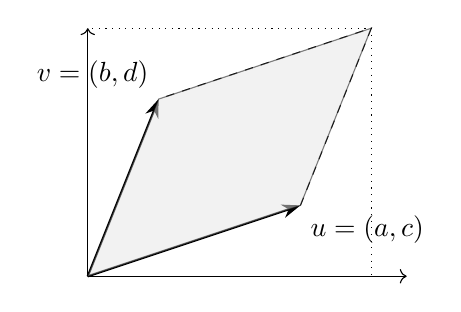
\begin{tikzpicture}[scale=0.9]
  \draw[->] (0,0) -- (4.5,0);
  \draw[->] (0,0) -- (0,3.5);
  \coordinate (O) at (0,0);
  \coordinate (U) at (3,1);
  \coordinate (V) at (1,2.5);
  \coordinate (W) at ($(U)+(V)$);
  \draw[thick,-{Stealth[]}] (O) -- (U) node[below right] {$u=(a,c)$};
  \draw[thick,-{Stealth[]}] (O) -- (V) node[above left] {$v=(b,d)$};
  \draw[dashed] (U) -- (W) -- (V);
  \draw[fill=gray!20,opacity=0.5] (O)--(U)--(W)--(V)--cycle;
  \draw[dotted] (0,0) rectangle (4,3.5);
\end{tikzpicture}
\end{center}

Enclose the parallelogram in the axis-aligned bounding box of width
$a+b$ and height $c+d$. The box consists of the parallelogram, two
right triangles with legs $a,c$ (combined area $ac$), two right
triangles with legs $b,d$ (combined area $bd$), and two $b\times c$
rectangles (combined area $2bc$). So
\[
(a+b)(c+d) = \text{Area} + ac + bd + 2bc
\quad\Longrightarrow\quad
\text{Area} = ad - bc.
\]

\begin{definition}
The \emph{determinant} of a matrix
$A=\begin{pmatrix}a&b\\c&d\end{pmatrix}$ is the \emph{signed} area
spanned by $u=(a,c)$, $v=(b,d)$. 
\end{definition}
We had just saw that $\det A = ad-bc$.
Geometrically: $\det A = 0$ exactly when the columns of $A$ are
parallel --- the parallelogram they span is flat, with zero area. 

\section{Eigenvalues of a $2\times 2$ matrix}

\begin{definition}
A nonzero vector $v$ is an \emph{eigenvector} of $A$ with
\emph{eigenvalue} $\lambda$ if $Av = \lambda v$.
\end{definition}

Rearranging, $(A-\lambda I)v = 0$ for some $v\ne 0$. We saw that
$(A-\lambda I)v$ is the combination of $(A-\lambda I)$'s two columns
weighted by $v$'s entries; for a \emph{nonzero} $v$ to give $0$, that
combination must be nontrivial, which is only possible if the two
columns are parallel, i.e.
\[
\det(A-\lambda I) = 0.
\]

\paragraph{Useful fact.}
The determinant is the product of eigenvalues, whereas the trace is
their sum.

\section{Eigendecomposition}
Suppose $A$ has eigenvectors $v_1,v_2$ with eigenvalues
$\lambda_1,\lambda_2$, and let $P=\begin{pmatrix}v_1 & v_2\end{pmatrix}$
(eigenvectors as columns). Then
\[
AP = \begin{pmatrix}Av_1 & Av_2\end{pmatrix}
   = \begin{pmatrix}\lambda_1 v_1 & \lambda_2 v_2\end{pmatrix}
   = PD, \qquad D=\begin{pmatrix}\lambda_1&0\\0&\lambda_2\end{pmatrix},
\]
so, if $v_1,v_2$ are independent ($P$ invertible),
\[
A = PDP^{-1}.
\]
$P$ is a \emph{change of basis}: $P^{-1}$ converts a vector from the
standard basis to \emph{eigenbasis} coordinates (coefficients along
$v_1,v_2$), and $P$ converts back. In eigenbasis coordinates $A$ acts
as the diagonal $D$.

\section{The determinant for a $3\times 3$ matrix}
\[
\det\begin{pmatrix}a_1&b_1&c_1\\a_2&b_2&c_2\\a_3&b_3&c_3\end{pmatrix}
= a_1\det\begin{pmatrix}b_2&c_2\\b_3&c_3\end{pmatrix}
- a_2\det\begin{pmatrix}b_1&c_1\\b_3&c_3\end{pmatrix}
+ a_3\det\begin{pmatrix}b_1&c_1\\b_2&c_2\end{pmatrix}.
\]
The same interpretations hold: the determinant is (signed) volume, the
determinant is the product of eigenvalues, and the trace is the sum of
eigenvalues.

\chapter{Linear ODEs}

\section{A single linear equation}
\[
\dot x = ax, \qquad x(0)=x_0.
\]
Solve: $\frac{d}{dt}\log x = \dot x/x = a$, so $\log x = \log x_0 + at$, i.e.
\[
x(t) = x_0 e^{at}.
\]
$a>0$: exponential growth. $a<0$: exponential decay. $a=0$: constant.

\section{Why linearity matters}
A system $\dot x = Ax$ ($x\in\mathbb{R}^n$, $A$ a matrix) is
\emph{linear} in $x$. Its key property: if $x_1(t), x_2(t)$ both solve
$\dot x = Ax$, so does any combination $c_1x_1+c_2x_2$, since
\[
\frac{d}{dt}(c_1x_1+c_2x_2) = c_1\dot x_1 + c_2\dot x_2 = c_1Ax_1+c_2Ax_2 = A(c_1x_1+c_2x_2).
\]

\section{Diagonal systems in two dimensions}
A \emph{diagonal} system decouples into two copies of
Section~1:
\[
\dot x = \lambda_1 x, \qquad \dot y = \lambda_2 y
\quad\Longrightarrow\quad
x(t)=x_0e^{\lambda_1 t},\ \ y(t) = y_0e^{\lambda_2 t}.
\]
The qualitative picture depends on the signs of $\lambda_1,\lambda_2$:

\begin{figure}[h]
\centering
\includegraphics[width=\linewidth]{visualizations/phase_portraits_real.pdf}
\caption{Both negative: every trajectory decays to the origin
  (\emph{stable node}). Both positive: every trajectory grows away
  from it (\emph{unstable node}). Opposite signs: the origin attracts
  along one axis and repels along the other (\emph{saddle}).}
\end{figure}

\section{Diagonal systems with complex eigenvalues}
Take $A = \begin{pmatrix}a&-b\\b&a\end{pmatrix}$, i.e.\
$\dot x = ax-by,\ \dot y = bx+ay$. Its eigenvalues solve
$\det(A-\lambda I)=(a-\lambda)^2+b^2=0$, so $\lambda = a\pm ib$:
complex. Set $z=x+iy$; then
\[
\dot z = \dot x+i\dot y = (ax-by)+i(bx+ay) = (a+ib)(x+iy) = (a+ib)z,
\]
the single linear equation of Section~1, now with complex $a+ib$.
Its solution is $z(t) = z_0e^{(a+ib)t} = z_0e^{at}\big(\cos bt +
i\sin bt\big)$: a rotation at rate $b$, scaled by $e^{at}$.

\begin{figure}[h]
\centering
\includegraphics[width=\linewidth]{visualizations/phase_portraits_complex.pdf}
\caption{$a<0$: spiral sink. $a=0$: pure rotation, a \emph{center}.
  $a>0$: spiral source.}
\end{figure}

\section{Every linear system is diagonal, in the right coordinates}
Let $A$ have eigenvectors $v_1,v_2$ (eigenvalues $\lambda_1,\lambda_2$,
possibly complex conjugates) and $P=\begin{pmatrix}v_1&v_2\end{pmatrix}$
as in the eigendecomposition $A=PDP^{-1}$. Write $x = Pu$, i.e.\ $u =
P^{-1}x$ gives the coordinates of $x$ in the eigenbasis. Then
\[
\dot u = P^{-1}\dot x = P^{-1}Ax = P^{-1}APu = Du.
\]
So $u$ solves a \emph{diagonal} system --- Section~3 if
$\lambda_1,\lambda_2$ are real, Section~4 if they are complex
conjugates --- and $x(t) = Pu(t)$ translates the solution back to the
original coordinates. Every linear system is, up to a change of basis,
one of the pictures above.

\chapter{The SIR Model, Continued}

\section{The threshold phenomenon}

Say the initial proportion of infecteds is $I(0) \ne 0$. Will the
infection \emph{invade}? I.e.~will $I$ increase? Equivalently, does
$\dot I>0$ hold?

\[
\dot I = \beta S I - \gamma I = I(\beta S - \gamma).
\]
So  $\dot{I} > 0$ if 
\[
\beta S - \gamma  > 0.
\]
We must have $\beta S - \gamma > 0$, or equivalently
\[
S > \frac{\gamma}{\beta}.
\]
So if $S<\gamma/\beta$ the infection cannot invade. The implication
for vaccination strategies and herd immunity is immediate.

\subsection{The basic reproduction number}
What is $\beta/\gamma$? Recall $1/\gamma$ is the average time to
recovery, i.e.\ the disease duration and $\beta$ is infections per
individual per time unit (in a fully susceptible population). Hence
$R_0$ is the expected number of secondary infections caused by a
single infected individual introduced into an otherwise fully
susceptible population. We denote it
\[
R_0 = \frac{\beta}{\gamma}
\]


\section{Demographics}
We want to include births and deaths. Individuals are born into the
susceptible class $S$ at rate $\mu$ (per unit of the whole population)
and die at the same per-capita rate $\mu$ from every class, so
population size is still fixed. The new equations are
\begin{align*}
\dot S &= \mu - \beta S I - \mu S, \\
\dot I &= \beta S I - \gamma I -\mu I, \\
\dot R &= \gamma I - \mu R.
\end{align*}
As before, $\dot S + \dot I + \dot R = 0$, so $S+I+R=1$ stays
constant.

\subsection{$R_0$ for an SIR model with demographics}
With demography, an infected individual leaves the infected class
either by recovering (rate $\gamma$) or by dying (rate $\mu$),
independently. Recall that \emph{minimum} of two independent
exponentials is exponential with the sum of rates, so the time spent
infected is $\text{Exp}(\gamma+\mu)$.

Using the same interpretation as before, $R_0$ is (contacts during
infection) $\times$ (transmission probability per contact) with the
mean infectious period $1/(\gamma+\mu)$:
\[
R_0 = \frac{\beta}{\gamma + \mu}.
\]

\section{Equilibria}
We find equilibrium states by equating the derivatives to zero.

\subsection{Equilibrium analysis for basic SIR model}

Recall the basic SIR model:
\begin{align*}
\dot S &= -\beta S I, \\
\dot I &= \beta S I - \gamma I, \\
\dot R &= \gamma I.
\end{align*}
Set all three derivatives to zero. $\dot R = \gamma I = 0$ forces
$I=0$ (since $\gamma>0$). Then  $\dot S = \dot{I} = 0$.

So the equilibria are $(S,0,R)$ for $S+R=1$ (and, of course, $0\le
S\le 1$). This is a \emph{disease-free equilibrium} (DFE).

\subsection{Equilibrium analysis for SIR model with demographics}

Recall the model with demography:
\begin{align*}
\dot S &= \mu - \beta S I - \mu S, \\
\dot I &= \beta S I - \gamma I - \mu I, \\
\dot R &= \gamma I - \mu R.
\end{align*}
Set all three derivatives to zero. From $\dot I=0$:
$I[\beta S-(\gamma+\mu)]=0$, so either $I=0$ or
$S=\dfrac{\gamma+\mu}{\beta}=\dfrac{1}{R_0}$.

\paragraph{Disease-free equilibrium (DFE).} Then $\dot S=\mu(1-S)=0$
forces $S=1$. Other compartments are empty.

\paragraph{Endemic equilibrium (EE).} Take $\dot I=0$. If $I = 0$ we are at DFE. So assume $I > 0$. Then
\[
\dot{I} = 0 \Rightarrow \beta S^* = \gamma + \mu \Rightarrow S^* = \frac{\gamma +\mu}{\beta} = \frac{1}{R_0}.  
\]
Then
\[
I^* = \frac{\mu}{\gamma+\mu}\left(1-\frac{1}{R_0}\right)
\]
and
\[
R^* = \frac{\gamma}{\gamma+\mu}\left(1-\frac{1}{R_0}\right).
\]
So
\[
(S^*,I^*,R^*) = \left(\frac{1}{R_0},\ \ \frac{\mu}{\gamma+\mu}\Big(1-\frac{1}{R_0}\Big),\ \ \frac{\gamma}{\gamma+\mu}\Big(1-\frac{1}{R_0}\Big)\right).
\]
Note that this equilibrium is feasible (i.e.\ $I^*>0$) exactly when
$R_0>1$.

\section{Stability analysis}

\subsection{Linearization}

For a real function of one variable, near a point $x^*$:
\[
f(x^*+\delta x) \approx f(x^*) + \frac{df}{dx}(x^*)\,\delta x.
\]
In two dimensions a function takes two inputs and produces two
outputs $(x,y)\mapsto (f(x,y),g(x,y))$. So:

\begin{align*}
f(x^*+\delta x,\,y^*+\delta y) &\approx f(x^*,y^*) + \frac{\partial f}{\partial x}\delta x + \frac{\partial f}{\partial y}\delta y \\
g(x^*+\delta x,\,y^*+\delta y) &\approx g(x^*,y^*) + \frac{\partial g}{\partial x}\delta x + \frac{\partial g}{\partial y}\delta y.
\end{align*}
Collecting:
\[
\begin{pmatrix} f(x^*+\delta x,y^*+\delta y) \\ g(x^*+\delta x,y^*+\delta y) \end{pmatrix}
\approx
\begin{pmatrix} f(x^*,y^*) \\ g(x^*,y^*) \end{pmatrix}
+
\begin{pmatrix} \partial f/\partial x & \partial f/\partial y \\ \partial g/\partial x & \partial g/\partial y \end{pmatrix}
\begin{pmatrix} \delta x \\ \delta y \end{pmatrix}.
\]

\begin{definition}
The \emph{Jacobian} of $(f,g)$ at $(x^*,y^*)$ is
\[
J(x^*,y^*) = \begin{pmatrix} \partial f/\partial x & \partial f/\partial y \\ \partial g/\partial x & \partial g/\partial y \end{pmatrix},
\]
\end{definition}
So:
\[
\begin{pmatrix} f(x^*+\delta x,y^*+\delta y) \\ g(x^*+\delta x,y^*+\delta y) \end{pmatrix}
\approx
\begin{pmatrix} f(x^*,y^*) \\ g(x^*,y^*) \end{pmatrix}
+
J(x^*, y^*) \begin{pmatrix} \delta x \\ \delta y \end{pmatrix}.
\]

Now, our goal is to linearize a dynamical system 
\[
\begin{pmatrix} \dot x \\ \dot y \end{pmatrix} = \begin{pmatrix} f(x,y) \\ g(x,y) \end{pmatrix}
\]
using the Jacobian. We linearize at an equilibrium point, $f(x^*,y^*)
= g(x^*,y^*) = 0$ and let $x=x^*+\delta x$, $y=y^*+\delta y$. Then
\begin{align*}
  \begin{pmatrix}
    \dot x \\ \dot y
  \end{pmatrix} &= \begin{pmatrix} f(x^*,y^*) \\ g(x^*,y^*) \end{pmatrix} \\
\end{align*}

Since $x^*,y^*$ are constant, $\dot x=\dot{\delta x}$ and $\dot
y=\dot{\delta y}$, so by the approximation above and using $f(x^*,y^*)
= g(x^*,y^*) = 0$:
\[
\begin{pmatrix} \dot{\delta x} \\ \dot{\delta y} \end{pmatrix}
\approx
J(x^*,y^*)
\begin{pmatrix} \delta x \\ \delta y \end{pmatrix}.
\]
Near an equilibrium, the dynamics of a small perturbation are
therefore approximately \emph{linear}, governed entirely by the
Jacobian.

\paragraph{Why is this useful?}
Stability of an equilibrium is ``stable'' determined by its
eigenvalues. Roughly, all eigenvalues have to be
negative\footnote{have negative real part.} for an equilibrium to be
stable.

\subsection{Linearization of SIR model}
Here the variables are $S$ and $I$:
\begin{align*}
\dot S &= f(S,I) := \mu(1-S)-\beta SI \\
\dot I &= g(S,I) := \beta SI - (\gamma+\mu)I\\ 
\end{align*}
The Jacobian is
\[
J(S,I) = \begin{pmatrix} -\mu-\beta I & -\beta S \\ \beta I & \beta S-(\gamma+\mu) \end{pmatrix}.
\]


\subsubsection{Linearization around the disease-free equilibrium (DFE)}
In the disease-free equilibrium $I^*=0$ and $S^*=1$:
\[
J(S^*, I^*) = \begin{pmatrix} -\mu & -\beta \\ 0 & \beta-(\gamma+\mu) \end{pmatrix}
\]
Eigenvalues are:
\[
\lambda_1 = -\mu, \qquad \lambda_2 = \beta-(\gamma+\mu) = (\gamma+\mu)(R_0-1).
\]
$\lambda_1<0$ always; $\lambda_2<0 \iff R_0<1$. So the disease-free
equilibrium is stable iff $R_0<1$.

\subsubsection{Linearization around the endemic equilibrium (EE)}
In the endemic equilibrium,
\[
(S^*,I^*,R^*) =
\left(\frac{1}{R_0},\ \ \frac{\mu}{\gamma+\mu}\Big(1-\frac{1}{R_0}\Big),\ \ \frac{\gamma}{\gamma+\mu}\Big(1-\frac{1}{R_0}\Big)\right).
 \]
$\beta S^*=\gamma+\mu$ and $\beta
I^*=\mu(R_0-1)$ and the Jacobian becomes
\[
J(S^*,I^*) = \begin{pmatrix} -\mu R_0 & -(\gamma+\mu) \\ \mu(R_0-1) & 0 \end{pmatrix},
\qquad
\operatorname{tr}J(S^*,I^*) = -\mu R_0, \qquad \det J(S^*,I^*) = \mu(\gamma+\mu)(R_0-1).
\]
For a $2\times 2$ matrix, both eigenvalues have negative real part iff
$\operatorname{tr}<0$ and $\det>0$. Here $\operatorname{tr}J^*<0$
always, and $\det J^*>0 \iff R_0>1$. So whenever the endemic
equilibrium exists ($R_0>1$), it is automatically stable.

\paragraph{Summary.}
$R_0<1 \Rightarrow$ disease-free equilibrium is stable. $R_0>1 \Rightarrow$ endemic equilibrium is stable.

\chapter{Simulating Infectious Diseases}

\section{Euler's method}

Recall $f(x+\Delta x) \approx f(x)+f'(x)\Delta x$. \emph{Euler's
method} uses this repeatedly for $\dot x = f(x,t)$:  
\[
x_{t+\Delta t} \approx x_t + f(x_t,t)\,\Delta t,
\]
then repeat. For an SIR system, $x_t = (S,I,R)$:
\begin{lstlisting}
import numpy as np

def euler(beta, gamma, dt, n):
    S, I = np.zeros(n), np.zeros(n)
    S[0], I[0] = 0.99, 0.01
    for t in range(n - 1):
        dS =  - beta * S[t] * I[t]
        dI = beta * S[t] * I[t] - gamma * I[t]

        # Euler's method: new state = old state + rate * step size
        S[t + 1] = S[t] + dS * dt
        I[t + 1] = I[t] + dI * dt
        
    return S, I
\end{lstlisting}

\section{Incidence vs.~prevalence}
$I_t$ is the per-capita \emph{prevalence}: the proportion infected at
a time $t$. Surveillance rarely measures prevalence. Instead,
surveillance efforts reoirt \emph{incidence}: the number of \emph{new}
infections over a reporting interval, e.g.\ a week:

\begin{definition}
The \emph{incidence} over an interval $[t-\Delta t,\,t]$ is the number
of new infections:
\[
\text{Incidence}(t) = N \int_{t-\Delta t}^{t} \lambda_s\, S_s \, ds.
\]
\end{definition}
Tyically we normalize to find the \emph{per-capita} incidence

\begin{lstlisting}
import numpy as np

def incidence_euler(beta, gamma, dt, k, n):
    S, I = 0.99, 0.01
    incidence = np.zeros(n)
 
    for t in range(n-1):
        for s in range(k):
            new_infections = beta * S * I
            dS =  - new_infections
            dI = new_infections - gamma * I

            # Euler's method: new state = old state + rate * step size
            S += dS * dt
            I +=  dI * dt

            # Accumulate new infections
            incidence[t+1] += new_infections * dt 
        
    return incidence
\end{lstlisting}

Note: since the Euler time step (e.g.~day) may differ from the
sampling rate\footnote{To be precise, the Euler step may differ from
the \emph{inverse} of the sampling rate.} (e.g.~one week) we had to
implement another loop that rubs over $0,...,k$.

\section{Log-transformations}

Working with $\log$ variables is more stable numeically. We can easily
find that

\begin{align*}
  \dot{\log(S)} &= \frac{1}{S} \dot{S}  \\
  &=  \frac{-\beta S I}{S} \\
  %&= -\beta I \\
  &= -\beta e^{\log(I)}\\ 
  \dot {\log(I)} &= \frac{\beta SI -\gamma I}{I} \\
  &= -\beta e^{\log(S)} - \gamma.
\end{align*}

\begin{lstlisting}
import numpy as np

def log_euler(beta, gamma, dt, n):
    logS, logI = np.zeros(n), np.zeros(n)
    logS[0], logI[0] = np.log(0.99), np.log(0.01) 
    for t in range(n - 1):
        dlogS =  - beta * np.exp(logI[t])
        dlogI = beta * np.exp(logS[t]) - gamma 

        # Euler's method: new state = old state + rate * step size
        logS[t + 1] = logS[t] + dlogS * dt
        logI[t + 1] = logI[t] + dlogI * dt
        
    return S, I
\end{lstlisting}



%% \section{Observation noise and process noise}

%% A simulated (or real) epidemic time series has two distinct sources
%% of randomness, and it matters which one you mean.

%% \begin{itemize}
%%   \item \textbf{Process noise}: randomness in the \emph{true}
%%   dynamics themselves --- e.g.\ random fluctuations in the contact
%%   rate. This perturbs the actual trajectory $S_t,I_t,R_t$, step by
%%   step, as it is generated.
%%   \item \textbf{Observation noise}: randomness in how that true state
%%   is \emph{measured} --- underreporting, test error, sampling. This
%%   is added only once, after the true trajectory is simulated, to
%%   produce the ``data'' we pretend to observe.
%% \end{itemize}
%% From data alone, the two are often hard to tell apart --- a central
%% difficulty in fitting epidemic models, and part of the motivation for
%% the methods we turn to at the end of this chapter.

\section{A driven epidemic model}

Many infectious diseases are seasonal (e.g.~measles and influenza),
since transmission varies in time. We let $\beta$ vary
periodically in time:
\[
\beta_t = \beta_0\big(1+\beta_1\cos(2\pi t)\big),
\]
This is a \emph{driven}, or \emph{forced} system, with $t$ in years,
$\beta_0>0$ the baseline transmission rate, and $\beta_1\in[0,1)$ the
amplitude of seasonal forcing. Substituting into the demographic SIR
system:
\begin{align*}
\dot S &= \mu(1-S) - \beta_t\, S I, \\
\dot I &= \beta_t\, S I - (\gamma+\mu) I, \\
\dot R &= \gamma I - \mu R.
\end{align*}
%% This is a purely deterministic system, driven by a perfectly periodic
%% $\beta_t$, with no noise anywhere --- yet, for suitable parameters, it
%% produces recurring outbreaks that are not all the same size:

\begin{figure}[h]
\centering
\includegraphics[width=0.8\linewidth]{visualizations/driven_sir.pdf}
\caption{\label{fig:driven_sir}A biennial cycle: one large outbreak (red), one small (blue),
repeating exactly every two years ($\log$ scale --- the small
outbreaks are $\sim\!15\times$ smaller). Parameters: $\mu=0.02\,\text{yr}^{-1}$,
$\gamma=365/13\,\text{yr}^{-1}$ (13-day infectious period), $R_0=17$
(so $\beta_0=R_0(\gamma+\mu)\approx477.6\,\text{yr}^{-1}$),
$\beta_1=0.185$.}
\end{figure}

%% \section{Adding an incubation stage: the SEIR model}
%% The SIR model above has no incubation period: a susceptible becomes
%% infectious immediately on contact. For measles this is unrealistic ---
%% symptoms (and infectiousness) begin only $\sim\!8$--$12$ days after
%% exposure. We add an \emph{exposed} (infected but not yet infectious)
%% compartment $E$:
%% \begin{align*}
%% \dot S &= \mu(1-S) - \beta_t\, S I, \\
%% \dot E &= \beta_t\, S I - (\mu+a) E, \\
%% \dot I &= a E - (\mu+\gamma) I, \\
%% \dot R &= \gamma I - \mu R,
%% \end{align*}
%% where $1/a$ is the mean latent period.

\section{Units}
Units are crucial in simulations and modeling. We first decide on time
unit (e.g.~year, month, week) and then derive parameters
accordingly. See Table~\ref{tab:units} for examples.

\begin{table}[h]
\centering
\footnotesize
\begin{tabular}{l p{10.5cm}}
\hline
description & value \\
\hline
recovery rate &
$\gamma = \frac{1}{13}\,\text{day}^{-1} = \frac{1}{13}\left(\frac{\text{year}}{365}\right)^{-1}= \frac{365}{13}\,\text{year}^{-1}$ \\
%
%
%
birth rate & 
$\mu = \frac{1}{50}\,\text{year}^{-1} = \frac{1}{50}\big(365\,\text{day}\big)^{-1} = \frac{1}{18250}\,\text{day}^{-1}$ \\
%
%
%
contact rate &
$\kappa = 10\,\text{day}^{-1} =10\left(\frac{\text{year}}{365}\right)^{-1} = 3650\,\text{year}^{-1}$
\\ \hline
\end{tabular}
\caption{Converting parameter values between day and year units, by
treating day and year as algebraic symbols (day $=$ year$/365$).}
\label{tab:units}
\end{table}

\chapter{State-Space Reconstruction}

\section{States and Dynamics}

Define $\phi_t :=2\pi t \bmod 2\pi$. If we know $S, I$ and $\phi$ at
one time point we fully know the future. The \emph{state-space} of the
system is
\[
\Omega = (S,I,\phi) \in \mathbb{R}^2\times \mathbb{S}^1.
\]
To find $\omega_{t+1} = (S_{t+1}, I_{t+1}, \phi_{t+1})$ from $\omega_t =
(S_t, I_t, \phi_t)$ we integrate the SIR equations. This \emph{law}
is encapsulated in an operator $T\omega_t = \omega_{t+1}$.

\begin{definition}
  A \emph{dynamical system} is a pair $(\Omega, T)$ where $\Omega$
  called the \emph{state-space} and $T:\Omega \to \Omega$ is the
  \emph{law} of the dynamics.
\end{definition}

\begin{figure}[h]
\centering
\begin{minipage}{0.48\linewidth}
\includegraphics[width=\linewidth]{visualizations/driven_sir.pdf}
\end{minipage}
\hfill
\begin{minipage}{0.48\linewidth}
\includegraphics[width=\linewidth]{visualizations/sir_state_space.pdf}
\end{minipage}
\caption{The trajectory of the driven SIR model in time (left) and in
  state-space $(S,I,\phi)$ (right). Same parameters as
  Figure~\ref{fig:driven_sir}, \textcolor{red}{red} = large outbreak
  year, \textcolor{blue}{blue} = small).}
\end{figure}

\subsection{Prediction}\label{subsec:pred}
Say we know $\omega_t$ and we have many records of $\omega_s,
s<t$. What we do not have is access to $T$ itself. How would we
predict $\omega_{t+1}$? Easy: find $t^\star = \arg\min_{s<t}
\|\omega_s - \omega_t\|$ and predict $\omega_{t+1} \approx
\omega_{t^\star +1}$.

\section{Takens' theorem}
\begin{definition}
  An \emph{observable} is a real-valued function $X:\Omega \to
  \mathbb{R}$. We usually abuse notation and write $X_t =
  X(\omega_t)$.
\end{definition}

In many applications we do not have access to neither $T$ nor to
$\Omega$. However, we may have records of some observable(s). Let
$X_t$ be an observed quantity (e.g.\ fraction of infecteds $I_t$), fix
a lag $L$ and an \emph{embedding dimension} $E$. The \emph{delay
vector} is
\[
x_t = \big(X_t,\,X_{t-L},\,\dots, X_{t-(E-1)L}\big).
\]
It is easiest to take $L$ to be the spacing between observations
(i.e.~inverse of the sampling rate).

\begin{theorem}[Takens, 1981]
Let $(\Omega, T)$ a dynamical system, $d=\dim \Omega$ and $X:\Omega
\to \mathbb{R}$ an observable, $L>0$ some lag, and $E>2d$. Then, generically, the
map $x_t \to \omega_t$ is a diffeomorphism (everywhere differentiable
with an inverse which is also everywhere differentiable). 
\end{theorem}
In lignt of Takens' Theorem, we call $x_t$ \emph{reconstructed
states}. We denote the set of all reconstruted states $M_X := \{x_s:
s\leq t\}$.

\subsection{Why $E>2d$? (dimension counting)}
The map $x_t\to\omega_t$ can fail in two ways, and both are ruled out
by a dimension count once $E>2d$.

\begin{itemize}
\item \textbf{Injectivity.} $x_s=x_t$ for $s\ne t$ means $E$ equations
  $X(\omega_{s-kL})=X(\omega_{t-kL})$, $k=0,\dots,E-1$, hold at once.
  These are imposed on the $2d$-dimensional space of pairs
  $(\omega_s,\omega_t)\in\Omega\times\Omega$. With $E>2d$ this is
  \emph{overdetermined} --- generically, more equations than degrees
  of freedom means no solutions.
\item \textbf{Immersion.} The map fails to be locally invertible at
  $\omega_t$ exactly when some direction $v\in T_{\omega_t}\Omega$ is
  killed by all $E$ copies of $dX$ pulled back along the orbit. Again,
  generically, requiring $E$ independent conditions to vanish on a
  space of dimension $d-1$ forces $v=0$ once $E>2d$.
\end{itemize}

%% Two honest caveats. First, ``generically'' is doing real work: making
%% it rigorous needs transversality theory (Sard's theorem), not just
%% counting --- we do not prove that here. Second, the count assumes
%% $\omega_{s-kL}$, $k=0,\dots,E-1$, are genuinely $E$ \emph{independent}
%% pieces of information; this fails exactly on periodic orbits of low
%% period, which is why Takens' hypotheses also constrain $T$ (finitely
%% many such orbits, with non-resonant eigenvalues), not just $X$.

\subsection{The Olsen--Schaffer attractor}
Takens' theorem implies we can \emph{see} the state space of a system
we are investigating: just plot the reconstructed states / delay
vectors. For the SEIR model with measles parameters (Aron \& Schwartz),
Olsen \& Schaffer (1990) reconstruct
$\big(I_t,I_{t-L},I_{t-2L}\big)$, $L=3$ months:

\begin{figure}[h]
\centering
\includegraphics[width=0.7\linewidth]{visualizations/os_attractor.pdf}
\caption{\label{fig:os_attractor}Reconstructed attractor of the
  seasonally forced SEIR model, measles parameters (Aron \& Schwartz,
  as used by Olsen \& Schaffer 1990): $m=0.02\,\text{yr}^{-1}$
  (birth/death rate), $a=35.84\,\text{yr}^{-1}$ (latent period),
  $g=100\,\text{yr}^{-1}$ (infectious period),
  $\beta_0=1800\,\text{yr}^{-1}$, $\beta_1=0.28$.}
\end{figure}

\subsection{Prediction, revisited}
We observe $X_s, 0\leq s\leq t$ and would like to forecast
$X_{t+1}$. We take an approach analogous to the one we took in
Section~\ref{subsec:pred}:
\begin{enumerate}
  \item Build $x_s = (X_s, X_{s-1},\dots, X_{s-(E-1)})$ for $ E-1 \leq s \leq t$.
  \item Find $\arg \min_{E-1 \leq s \leq t} \|x_s - x_t\|$.
  \item Forecast $X_{s+1}$.
\end{enumerate}

How far ahead can this work? Take two states that start out
neighbors on the attractor and just let both evolve --- no
re-forecasting --- and track how far apart they drift as a function
of lead time:

\begin{figure}[h]
\centering
\includegraphics[width=0.7\linewidth]{visualizations/nn_prediction.pdf}
\caption{\label{fig:nn_prediction}RMSE (on $\log_{10}I$) between two
  initially-neighboring trajectories, as a function of forecast
  horizon. Same reconstructed state space and parameters as
  Figure~\ref{fig:os_attractor}. Growth is monotonic: nearby states on
  a chaotic attractor diverge, which is exactly what bounds how far
  ahead \emph{any} forecaster --- nearest-neighbor or otherwise --- can
  see.}
\end{figure}


\chapter{Convergent Cross Mapping}

\section{Skew products}

Suppose $X$ drives $Y$ but not vice versa. We can write this as a set of ODEs:
\begin{align*}
\dot X = f(X), & \qquad \dot Y = g(Y,X).
\end{align*}
Or, we can write this as abstract dynamical systems:
\begin{align*}
  \Omega^{X} = (\omega_1^{X},\dots, \omega_k^{X})& \qquad \Omega^Y = (\omega_1^{X},\dots, \omega_k^{X}, \omega^Y_{k+1}, \dots, \omega^Y_q),
\end{align*}
with dynamics operators $T^X$ and $T^Y$.  This is a \emph{skew
product}: $X$ evolves on its own; $Y$'s history depends on $X$'s. We
call $X$ the \emph{base} and $Y$ is called the \emph{fibre}. By
Takens' theorem applied to $Y$, the reconstructed manifold $M_Y \cong
\Omega^Y$ embeds information about $X$ as well as information about
$Y$. The converse reconstruction $M_X$ does \emph{not} contain
information about $Y$, since $X$ never sees $Y$.

\section{Causality}

\begin{definition}
We say that $X$ \emph{causally forces} $Y$ if $X,Y$ form a skew
product where $X$ is the base and $Y$ is the fibre.
\end{definition}

Operationally: can we find $\omega^X$ from $\omega^Y$? Or, can we do
the same using reconstructed states, i.e.~find $x_t$ from
$y_t$. Importantly, this does not necessitate knowing the law or
state-space of the dynamics.

\section{Convergent Cross Mapping}

Fix library length $L\le N$. For each $t$ in $1,\dots,L$:
\begin{enumerate}[nosep]
\item Find the $E+1$ nearest neighbors of $M_Y(t)$ among
  $\{M_Y(1),\dots,M_Y(L)\}\setminus\{M_Y(t)\}$, with time indices
  $t_1,\dots,t_{E+1}$.
\item Weight them by distance: $w_i \propto
  e^{-d(M_Y(t),M_Y(t_i))/d(M_Y(t),M_Y(t_1))}$.
\item Cross-map: $\hat X_t = \sum_i w_i\, X_{t_i}$.
\end{enumerate}
Skill: $\rho_L = \operatorname{corr}\big(\hat X,X\big)$ over $t=1,\dots,L$.

\paragraph{Convergence.} Plot $\rho_L$ vs.\ $L$. If $\rho_L$ increases
and plateaus as $L$ grows, $X$ causally forces $Y$: more of $Y$'s
history fills in $M_Y$ more completely, so nearby points on $M_Y$
genuinely share nearby $X$-states. A flat or non-increasing $\rho_L$
is evidence against causation, even if $X,Y$ are correlated ---
convergence, not correlation, is the signature.


\chapter{Attractor Dimension}

\section{What is a dimension}
Spread points uniformly across the real line and count how many fall
within a distance of $r$ from the origin. That number scales as $N(r) \sim r$.

Spread points uniformly across the plane and count how many fall
within a distance of $r$ from the origin. That number scales as $N(r) \sim r^2$.

Spread points uniformly across space and count how many fall within a
distance of $r$ from the origin. That number scales as $N(r) \sim r^3$.

For any $D$ dimensional object, if we spread points uniformly in it
and count how many are less than a distance $r$ from any particular
point ---that number scales as $N(D) \sim r^D$.

Say we obeserve points in $\mathbb{R}^n$. Count their number in $r$
balls. Then
\[
N(r) \sim r^D \Rightarrow D \approx \frac{\log N(r)}{\log r}
\]

\section{Correlation dimension}

\begin{definition}[Correlation sum]
For points $\{x_i\}_{i=1}^N$ on the attractor,
\[
C(r) = \frac{1}{N^2}\#\{(i,j): \|x_i-x_j\|<r\}.
\]
\end{definition}
As $r\to 0$, $C(r)\sim r^{D_C}$; the \emph{correlation dimension}
$D_C$ is the slope of $\log C(r)$ vs.\ $\log r$ (Grassberger \&
Procaccia, 1983).

For the Olsen--Schaffer attractor (lagged $\log_{10} I$ --- raw $I$'s
huge dynamic range, fine for viewing the attractor, washes out the
scaling plateau here):

\begin{center}
\includegraphics[width=0.6\linewidth]{visualizations/correlation_dimension.pdf}
\end{center}
$D_C\approx 2.33$, close to Olsen \& Schaffer's own estimate
($D_C\approx 2.52$ for this model).

\section{Levina--Bickel MLE estimator}

A second estimator, from the spacing of the $k$ nearest neighbors.
For point $x_i$ with neighbor distances $T_1(x_i)\le\cdots\le T_k(x_i)$:
\[
\hat m_k(x_i) = \left[\frac{1}{k-1}\sum_{j=1}^{k-1}
\log\frac{T_k(x_i)}{T_j(x_i)}\right]^{-1}.
\]
Average $\hat m_k(x_i)$ over $i$ and over a range of $k$ (here
$k=10,\dots,20$) for stability (Levina \& Bickel, 2004). On the same
attractor: $\hat D_{\mathrm{MLE}}\approx 2.48$ --- consistent with
$D_C$ above.



\end{document}
